\documentclass[conference]{IEEEtran}
\IEEEoverridecommandlockouts
\usepackage{graphicx}
\usepackage{amsmath}
\usepackage{amssymb}
\usepackage{booktabs}
\usepackage{tabularx}
\usepackage{xcolor}
\usepackage{tikz}
\usepackage[colorlinks=true,citecolor=red,urlcolor=black,linkcolor=green!45!black]{hyperref}
\usepackage[T1]{fontenc}
\usepackage{microtype}

\usetikzlibrary{arrows.meta,positioning,fit,backgrounds}

\newcommand{\fense}{\textsc{Fense}}
\newcommand{\clapenc}{\textsc{Clap}}
\newcommand{\sys}{\textsc{ClapCap}}

\renewcommand{\topfraction}{0.95}
\renewcommand{\bottomfraction}{0.95}
\renewcommand{\textfraction}{0.05}
\renewcommand{\floatpagefraction}{0.8}
\renewcommand{\dbltopfraction}{0.95}
\renewcommand{\dblfloatpagefraction}{0.8}
\setcounter{totalnumber}{6}
\setcounter{topnumber}{4}
\setcounter{dbltopnumber}{4}

\begin{document}

\title{ClapCap: CLAP Prefix for Music Captioning}

\author{\IEEEauthorblockN{Ali Ozkaya}
\IEEEauthorblockA{Department of Computer Engineering\\
İzmir Institute of Technology, İzmir, Turkey\\
aliozkaya@std.iyte.edu.tr\\
aliozkaya00@gmail.com}
\and
\IEEEauthorblockN{Prof.\ Dr.\ Aytu\u{g} Onan}
\IEEEauthorblockA{Department of Computer Engineering\\
İzmir Institute of Technology, İzmir, Turkey\\
aytugonan@iyte.edu.tr}
\thanks{979-8-3195-2149-1/26/\$31.00~\copyright2026 IEEE}}

\maketitle

\begin{abstract}
A useful music caption names genre, instrumentation and mood rather than discrete sound events.
We ask how far a lightweight language model can go when its only view of the audio is a short
learned prefix projected from a frozen embedding. \sys{} is the audio analogue of the ClipCap
image-captioning recipe: a frozen \clapenc{} encoder produces one clip embedding, a small MLP
maps it to a fixed-length prefix of pseudo-tokens, and a pretrained language model decodes the
caption. On MusicCaps we compare GPT-2 (124M, decoder-only) with T5-base (220M,
encoder--decoder), holding the encoder, projection, data split and evaluation fixed, and we
measure a per-model noise floor over three seeds so that every ablation delta is judged against
run-to-run variance. The two models are statistically indistinguishable at baseline
(\fense{} $0.400$ vs.\ $0.395$; noise floors $\pm0.014$ and $\pm0.035$), and second-stage
fine-tuning erases the differences introduced in the projection. The largest decoding lever
lifts \fense{} to $0.580$ almost entirely by removing the fluency-error term rather than by
improving semantics. Swapping the general frontend for music-specialised encoders helps only
where pretraining is pooled and joint audio--text. Against zero-shot reference captioners scored
on the identical split, the pipeline is the strongest leakage-free system, and a pairwise human
and LLM-as-judge study recovers a GPT-2-over-T5 preference that the automatic metrics call a
tie. Every experiment runs on a single consumer GPU.
\end{abstract}

\begin{IEEEkeywords}
Music captioning, audio--language models, prefix conditioning, CLAP, controlled ablation,
evaluation metrics
\end{IEEEkeywords}

\section{Introduction}

Most audio captioning research targets \emph{general} sound --- environmental events and
acoustic scenes --- on AudioCaps~\cite{kim2019audiocaps} and Clotho~\cite{drossos2020clotho}.
Music is different: a useful music caption describes genre, instrumentation, mood, tempo and
structure rather than discrete events. This work asks a deliberately minimal question: can a
lightweight language model recover music semantics from a simple projection of a frozen audio
embedding?

Our approach, \sys{}, adapts ClipCap~\cite{mokady2021clipcap}, which captions images by
projecting a frozen CLIP embedding into a prefix of pseudo-tokens for GPT-2. We replace the
image encoder with a frozen \clapenc{} audio encoder~\cite{wu2023clap}, caption music instead of
images, and turn the single-model recipe into a \emph{controlled comparison}: because the
encoder, projection, data split and evaluation are shared, the language model is the only thing
that changes between conditions. The contributions are:

\begin{itemize}\itemsep2pt
  \item an audio adaptation of the prefix-captioning recipe to music, with a
        \emph{noise-floor} methodology --- per-model run-to-run variance from three seeds ---
        so that single-run ablation deltas are interpretable rather than anecdotal;
  \item a controlled comparison of a decoder-only (GPT-2) and an encoder--decoder (T5) language
        model, with ablations over projection architecture, decoding strategy and the frozen
        audio frontend, each judged against that floor;
  \item a leakage-aware comparison against zero-shot reference captioners scored on the
        identical test split and harness, separating honest scores from training-on-test
        artifacts; and
  \item a pairwise human and LLM-as-judge study measuring agreement across lay listeners,
        audio-grounded models and text-only models.
\end{itemize}

We do not claim state of the art. Published captioning systems are evaluated on different
datasets with different reference counts, so a numerical comparison across them would be
meaningless; the contribution is the controlled analysis itself, together with the efficiency of
the recipe --- only a small projection, plus the language model, is trained.

\section{Related Work}\label{ch:related}

\textbf{Prefix captioning.} ClipCap~\cite{mokady2021clipcap} maps a frozen CLIP image embedding
to a constant-length prefix consumed by GPT-2, training only a small mapping network. It offers
a lightweight transformer mapper with a frozen LM and an MLP mapper with a fine-tuned LM;
\sys{} is the audio analogue of the latter. Notably, ClipCap reports that this variant
\emph{overfits} as trainable capacity grows --- an observation we recover, amplified, when
scaling the LM. In the audio domain, Pengi~\cite{deshmukh2023pengi} likewise conditions a small
LM on an audio-derived prefix, framing audio tasks as text generation.

\textbf{Music captioning.} MusicCaps~\cite{agostinelli2023musiclm} is a hand-curated set of
5{,}521 ten-second clips from AudioSet~\cite{gemmeke2017audioset}, each annotated by musicians.
LP-MusicCaps~\cite{doh2023lpmusiccaps} addresses caption scarcity by generating pseudo-captions
with an LLM over tag datasets. Such domain captioners, together with
BLAP~\cite{lanzendorfer2025blap}, are a natural \emph{reference} for \sys{}, and we score them
on our exact split in Section~\ref{sec:reference}.

\textbf{Audio language models.} End-to-end audio LLMs such as
Qwen2-Audio~\cite{chu2024qwen2audio}, Audio Flamingo~\cite{ghosh2026afnext} and
SALMONN~\cite{tang2024salmonn} couple a large LM to an audio encoder and are trained on large
instruction corpora. They are far heavier than the present recipe and bypass the
frozen-encoder/learned-prefix design we study, so we treat them as zero-shot references rather
than controlled comparisons.

\section{Method}\label{ch:method}

A clip is encoded once by a frozen \clapenc{} model into a $d_a$-dimensional embedding. A
projection network $f_\theta$ maps this vector to a prefix
$p_1,\dots,p_k \in \mathbb{R}^{d_{\text{lm}}}$ of $k$ pseudo-tokens in the LM embedding space,
and the LM generates the caption autoregressively, conditioned on that prefix
(Figure~\ref{fig:pipeline}).

\begin{figure*}[!t]\centering
\footnotesize
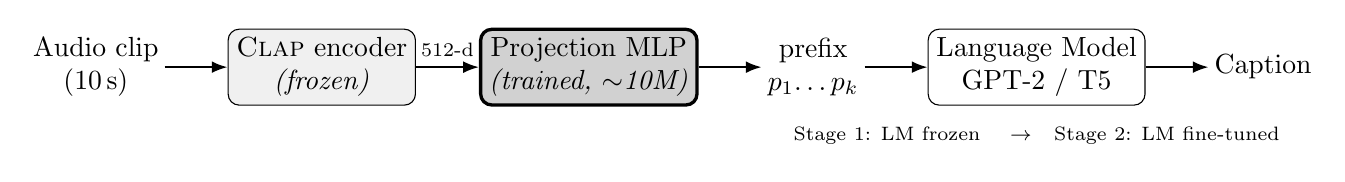
\begin{tikzpicture}[
    node distance=5mm and 8mm,
    box/.style={draw, rounded corners, minimum height=8mm, align=center, inner sep=3pt},
    frozen/.style={box, fill=black!6},
    trained/.style={box, fill=black!18, very thick},
    data/.style={align=center, inner sep=2pt},
    flow/.style={-{Latex[length=2mm]}, thick}]
  \node[data] (audio) {Audio clip\\(10\,s)};
  \node[frozen, right=of audio] (clap) {\clapenc{} encoder\\\emph{(frozen)}};
  \node[trained, right=of clap] (proj) {Projection MLP\\\emph{(trained, $\sim$10M)}};
  \node[data, right=of proj] (prefix) {prefix\\$p_1\!\dots p_k$};
  \node[box, right=of prefix] (lm) {Language Model\\GPT-2 / T5};
  \node[data, right=of lm] (cap) {Caption};
  \draw[flow] (audio) -- (clap);
  \draw[flow] (clap) -- node[above,font=\scriptsize]{512-d} (proj);
  \draw[flow] (proj) -- (prefix);
  \draw[flow] (prefix) -- (lm);
  \draw[flow] (lm) -- (cap);
  \node[font=\scriptsize, below=1.5mm of lm, align=center]
       {Stage~1: LM frozen \quad$\rightarrow$\quad Stage~2: LM fine-tuned};
\end{tikzpicture}
\caption{The \sys{} pipeline. A frozen \clapenc{} encoder turns the clip into a single 512-d
embedding; a small projection MLP --- the only newly added module --- maps it to a $k$-token
prefix in the LM embedding space; the LM generates the caption. Stage~1 trains the projection
with the LM frozen; Stage~2 additionally fine-tunes the LM.}
\label{fig:pipeline}
\end{figure*}

\textbf{Audio encoder.} We use the LAION checkpoint \texttt{laion/clap-htsat-unfused}
\cite{wu2023clap}, whose audio tower is an HTS-AT transformer~\cite{chen2022htsat} producing a
512-dimensional embedding. \clapenc{} is trained on general audio and is \emph{not}
music-specialised --- a deliberate test of how far a general frontend carries on a music task,
which Section~\ref{sec:encoder} then probes directly. Embeddings are precomputed once and
cached, so the encoder never runs during training or evaluation.

\textbf{Projection and language models.} The projection is a small MLP,
$\text{Linear}\!\rightarrow\!\text{LayerNorm}\!\rightarrow\!\text{GELU}\!\rightarrow\!
\text{Dropout}\!\rightarrow\!\text{Linear}$, reshaped to $(k,d_{\text{lm}})$, with baseline
prefix length $k{=}8$, dropout $0.3$ and depth $2$. We compare
GPT-2~\cite{radford2019gpt2} (decoder-only, 124M) and T5-base~\cite{raffel2020t5}
(encoder--decoder, 220M); for T5 the prefix is fed to the encoder, for GPT-2 it is prepended as
input embeddings.

\textbf{Two-stage training.} In Stage~1 the LM is frozen and only the projection is trained; in
Stage~2 the projection and the full LM are fine-tuned together, the audio encoder staying
frozen. These correspond to ClipCap's frozen-LM and fine-tuned-LM regimes. The objective in both
stages is autoregressive cross-entropy on caption tokens conditioned on the prefix,
\[
  \mathcal{L} = -\sum_{j}\log p_\theta\!\left(c_j \mid p_1,\dots,p_k, c_1,\dots,c_{j-1}\right).
\]
We use AdamW~\cite{loshchilov2019adamw} (weight decay $0.1$), cosine
annealing~\cite{loshchilov2017sgdr}, batch size $8$ and early stopping (patience $5$). Per
model only the learning rates are tuned, via a 16-trial Optuna~\cite{akiba2019optuna} search
over an eight-epoch proxy; everything else is fixed so the LM stays the controlled variable.

\textbf{Efficiency.} The only newly added module is the projection ($\sim$$10.2$M parameters).
The complete model is 124M (GPT-2) or 220M (T5) parameters --- one to two orders of magnitude
smaller than billion-parameter end-to-end audio LLMs --- and every experiment in this paper runs
on a single consumer GPU (NVIDIA RTX~5090).

\section{Experimental Study}\label{ch:experiments}

\subsection{Setup}

All experiments run on one workstation with an NVIDIA RTX~5090, using PyTorch, HuggingFace
\texttt{transformers}, Optuna, and the \texttt{aac-metrics} package for evaluation. We use
MusicCaps~\cite{agostinelli2023musiclm} with a fixed three-way random split: a held-out test set
($n{=}529$, final metrics only), a validation set ($n{\approx}495$) for checkpoint selection and
hyperparameter search, and the remainder for training ($n{\approx}4{,}455$). The split seed is
fixed across all conditions, so every model and seed is scored on the identical test set.

A single shared harness scores all conditions with BLEU-1 and BLEU-4~\cite{papineni2002bleu},
METEOR~\cite{banerjee2005meteor}, ROUGE-L~\cite{lin2004rouge}, CIDEr-D~\cite{vedantam2015cider},
SPICE~\cite{anderson2016spice}, SPIDEr~\cite{liu2017spider}, SBERT-sim, FER and \fense{}.
\fense{}~\cite{zhou2022fense} is our primary metric: it combines a
Sentence-BERT~\cite{reimers2019sbert} semantic similarity with a fluency-error penalty (FER),
making it sensitive to the semantic correctness a listener cares about. No post-processing is
applied by default; sentence trimming is treated as an explicit decoding ablation
(Section~\ref{sec:decoding}).

To judge whether a delta is real, we retrain each baseline with three seeds
($42,43,44$), varying only initialisation, shuffling and dropout while holding the split fixed.
The standard deviation of each metric across seeds is our \emph{noise floor}; deltas smaller
than it are not interpreted as effects.

\subsection{Baseline comparison}\label{sec:baseline}

Table~\ref{tab:baseline} reports greedy-decoding test metrics with per-model noise floors. GPT-2
leads on nine of the ten metrics, including the primary \fense{} ($0.3998$ vs.\ $0.3954$); the
exception is FER, where T5 is lower (better), though that gap ($0.023$) sits inside T5's own FER
noise floor ($\pm0.0511$). The \fense{} margin ($0.004$) is likewise smaller than either model's
\fense{} noise floor ($\pm0.0137$ for GPT-2, $\pm0.0345$ for T5). We therefore do \emph{not}
read it as evidence that one architecture is better at music captioning under this recipe. The
noise floor is also $\sim$$2.5\times$ larger for T5 than for GPT-2, so the encoder--decoder is
noticeably noisier run-to-run and each model must be judged against its \emph{own} variance.

\begin{table*}[!t]
\centering
\caption{Baseline (greedy) test-set metrics per model, with $\pm$ run-to-run standard deviation
over three seeds (the noise floor). Best per column in bold; all metrics are higher-is-better
except FER.}
\label{tab:baseline}
\footnotesize
\setlength{\tabcolsep}{4pt}
\begin{tabular}{lrrrrrrrrrr}
\toprule
Model & BLEU-1 $\uparrow$ & BLEU-4 $\uparrow$ & METEOR $\uparrow$ & ROUGE-L $\uparrow$ &
CIDEr-D $\uparrow$ & SPICE $\uparrow$ & SPIDEr $\uparrow$ & SBERT-sim $\uparrow$ &
FER $\downarrow$ & \fense{} $\uparrow$ \\
\midrule
GPT-2 & \textbf{0.3091} & \textbf{0.0631} & \textbf{0.1265} & \textbf{0.2329} &
\textbf{0.1109} & \textbf{0.1091} & \textbf{0.1100} & \textbf{0.5820} & 0.3478 &
\textbf{0.3998} \\
 & \scriptsize$\pm$0.0019 & \scriptsize$\pm$0.0039 & \scriptsize$\pm$0.0041 &
\scriptsize$\pm$0.0017 & \scriptsize$\pm$0.0076 & \scriptsize$\pm$0.0032 &
\scriptsize$\pm$0.0024 & \scriptsize$\pm$0.0089 & \scriptsize$\pm$0.0272 &
\scriptsize$\pm$0.0137 \\
T5 & 0.3003 & 0.0574 & 0.1162 & 0.2275 & 0.0847 & 0.0866 & 0.0857 & 0.5564 &
\textbf{0.3251} & 0.3954 \\
 & \scriptsize$\pm$0.0122 & \scriptsize$\pm$0.0048 & \scriptsize$\pm$0.0036 &
\scriptsize$\pm$0.0027 & \scriptsize$\pm$0.0181 & \scriptsize$\pm$0.0124 &
\scriptsize$\pm$0.0149 & \scriptsize$\pm$0.0170 & \scriptsize$\pm$0.0511 &
\scriptsize$\pm$0.0345 \\
\bottomrule
\end{tabular}
\end{table*}

\begin{figure*}[!t]\centering
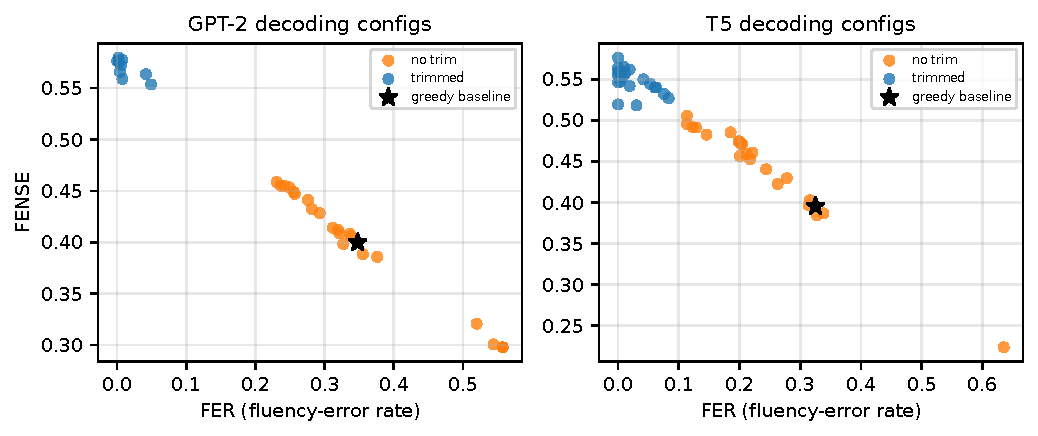
\includegraphics[width=\textwidth]{figures/fig_decoding_fense_fer.pdf}
\caption{\fense{} vs.\ FER over all decoding configurations. The near-perfect inverse trend
shows that \fense{} here is dominated by the fluency-error term: trimmed configurations (low
FER) score high \fense{} without improving semantic similarity. The star is greedy decoding.}
\label{fig:fensefer}
\end{figure*}

\subsection{Training stages and projection architecture}\label{sec:arch}

In Stage~1, where only the projection is trained, the projection configurations spread widely in
validation loss (a range of $0.38$ for GPT-2 and $0.83$ for T5). After Stage~2 that spread
collapses to $0.03$ for both models --- an $11\times$ reduction for GPT-2 and $31\times$ for T5:
full fine-tuning largely erases the architectural differences introduced by the projection. The
Stage-2 curves also show early overfitting, with validation loss bottoming within a few epochs,
which early stopping handles.

Consistently with that collapse, varying prefix length ($\{4,16\}$ around $8$), dropout
($\{0.1,0.5\}$ around $0.3$) and projection depth ($\{1,3\}$ around $2$) --- retraining each from
scratch --- leaves almost every configuration inside the baseline $\pm$ noise-floor band: no
projection hyperparameter reliably moves the primary metric for GPT-2. For T5 the prefix
variants produce larger \fense{} swings, but these coincide with collapses in the fluency-error
term rather than genuine semantic gains, as the next section explains.

\subsection{Decoding ablations}\label{sec:decoding}

Decoding strategies are evaluated on the fixed baseline checkpoint without retraining, isolating
generation behaviour. The dominant lever is trimming trailing incomplete sentences: it lifts
\fense{} from $0.3998$ to $0.5796$ for GPT-2 and from $0.3954$ to $0.5762$ for T5.

This gain is, however, \emph{largely an artifact of the metric}. Figure~\ref{fig:fensefer} plots
\fense{} against FER across all decoding configurations: the relationship is almost perfectly
inverse, and the trimmed configurations simply drive FER to near zero while the lexical metrics
barely move. Trimming removes the fluency penalty inside \fense{} without making captions
semantically more correct. We report it as a useful decoding choice for producing clean
captions, but caution against reading the headline \fense{} jump as a semantic improvement.

\subsection{Audio-encoder ablation}\label{sec:encoder}

The second axis keeps the language model fixed (GPT-2) and swaps the frozen \clapenc{} encoder
for music-specialised alternatives, re-extracting the cached embeddings and re-running the
learning-rate search per encoder while leaving the projection, training protocol and evaluation
untouched. Because Stage~2 erases upstream differences (Section~\ref{sec:arch}), we run this
comparison at Stage~1, where the frontend signal is most exposed, and replicate every encoder
over the three noise-floor seeds.

Against the general-audio baseline \texttt{clap-htsat-unfused} ($0.264\pm0.018$ \fense{}) we
compare two music \clapenc{} checkpoints, two MERT variants~\cite{li2024mert},
MusicFM~\cite{won2024musicfm}, and the self-supervised MuQ and MuQ-MuLan~\cite{zhu2025muq}. Only
two encoders clear the baseline band: \texttt{clap-music-speech} ($0.325\pm0.027$) and
\texttt{muq-mulan} ($0.321\pm0.008$). The remaining five --- including the frame-level
self-supervised MERT, MusicFM and MuQ, the last of which leads the MARBLE music-understanding
benchmark --- are not separable from general \clapenc{} at this stage. What survives is
therefore the \emph{pooled joint audio--text} pretraining shared by the two clearers, not raw
self-supervised acoustic features: at the frozen-projection stage, a CLAP-style clip embedding
is what the projection can exploit.

\subsection{Vocalist bias}\label{sec:qual}

The models reliably recover genre, instrumentation and mood, but two failure modes recur: on
non-music audio the pipeline still emits a confident music caption, and greedy decoding
occasionally degenerates into repetition. Most strikingly, both models tend to insert ``a male
vocalist singing melodically'' even when the reference states there is no singer.

The bias is \emph{not} a blind spot. GPT-2 mentions vocals on 95\% of clips whose reference
describes singing, but also on 43\% of clips marked instrumental (T5: 82\%\,/\,29\%) --- both
track vocal presence well above chance while skewing toward false positives. The skew mirrors
the training captions, of which 53\% mention vocals and in which male vocalists outnumber female
ones 2.2:1; the phrase ``male vocalist'' appears in 10\% of training captions but in roughly half
of the generated ones. Gender is worse: on references describing a \emph{female} singer, T5
outputs ``male'' 89\% of the time and GPT-2 44\%, while male references are almost never
misgendered (2--4\%). These rates persist across decoding configurations. Probing the frozen
\clapenc{} embeddings with zero-shot text prompts separates vocal from instrumental at 74\%
accuracy and vocalist gender at 76\%, so the embedding carries the cue but noisily; since both
LMs read the \emph{same} embedding, the gap between GPT-2 (56\%) and T5 (11\%) in
female-vocalist accuracy shows the failure is largely model-side. The bias is caption-prior
amplification under uncertain audio evidence, not a missing audio cue.

\subsection{Comparison with reference captioners}\label{sec:reference}

To place the pipeline against existing systems without an invalid cross-dataset comparison, we
score zero-shot reference captioners on the \emph{same} MusicCaps test split through the same
harness. These models ingest raw audio and bypass the \clapenc{}--projection--LM design, so they
are an external reference, not controlled ablation rows. They span general audio-LMs --- Audio
Flamingo (the AF-Next captioner checkpoint)~\cite{ghosh2026afnext},
Qwen2-Audio~\cite{chu2024qwen2audio} and a Qwen3-Omni captioner~\cite{xu2025qwen3omni} --- and
music-domain captioners --- LP-MusicCaps~\cite{doh2023lpmusiccaps} and
BLAP~\cite{lanzendorfer2025blap}. Figure~\ref{fig:reference_fense} summarises the primary metric.

Leakage is the central caveat. Several references may have seen MusicCaps in training:
Qwen2-Audio attains the highest \fense{} ($0.665$) but \emph{sweeps every metric including the
lexical ones}, the signature of training on the target captions; the MusicCaps-fine-tuned
LP-MusicCaps (transfer) reaches \fense{} $0.702$ with a CIDEr-D of $3.733$ --- an order of
magnitude above any honest row --- which is train-on-test memorisation, since ${\sim}48\%$ of
our random test split falls in its official-train set. We mark such rows with a dagger and,
where a model was fine-tuned on MusicCaps-train, additionally report a leakage-free
\emph{held-out} score on the MusicCaps-official-eval subset ($n{=}284$).

Among \emph{leakage-free} rows the lightweight pipeline is competitive: GPT-2 at its best
decoding configuration reaches \fense{} $0.580$, the highest non-leaked score, ahead of every
clean reference --- LP-MusicCaps (pretrain, MSD-only) at $0.378$, BLAP held-out at $0.476$, and
LP-MusicCaps transfer held-out at $0.543$. The general audio-LMs are fluent but off-style: Audio
Flamingo scores well on semantics (\fense{} $0.440$, SBERT-sim $0.586$) yet loses every lexical
metric to the trained pipeline, and the 30B Qwen3-Omni captioner is the weakest reference
(\fense{} $0.396$). A small model trained on-target matches the MusicCaps caption style that
large zero-shot models miss, and only models that have arguably seen the data score clearly
higher.

\begin{figure*}[!t]\centering
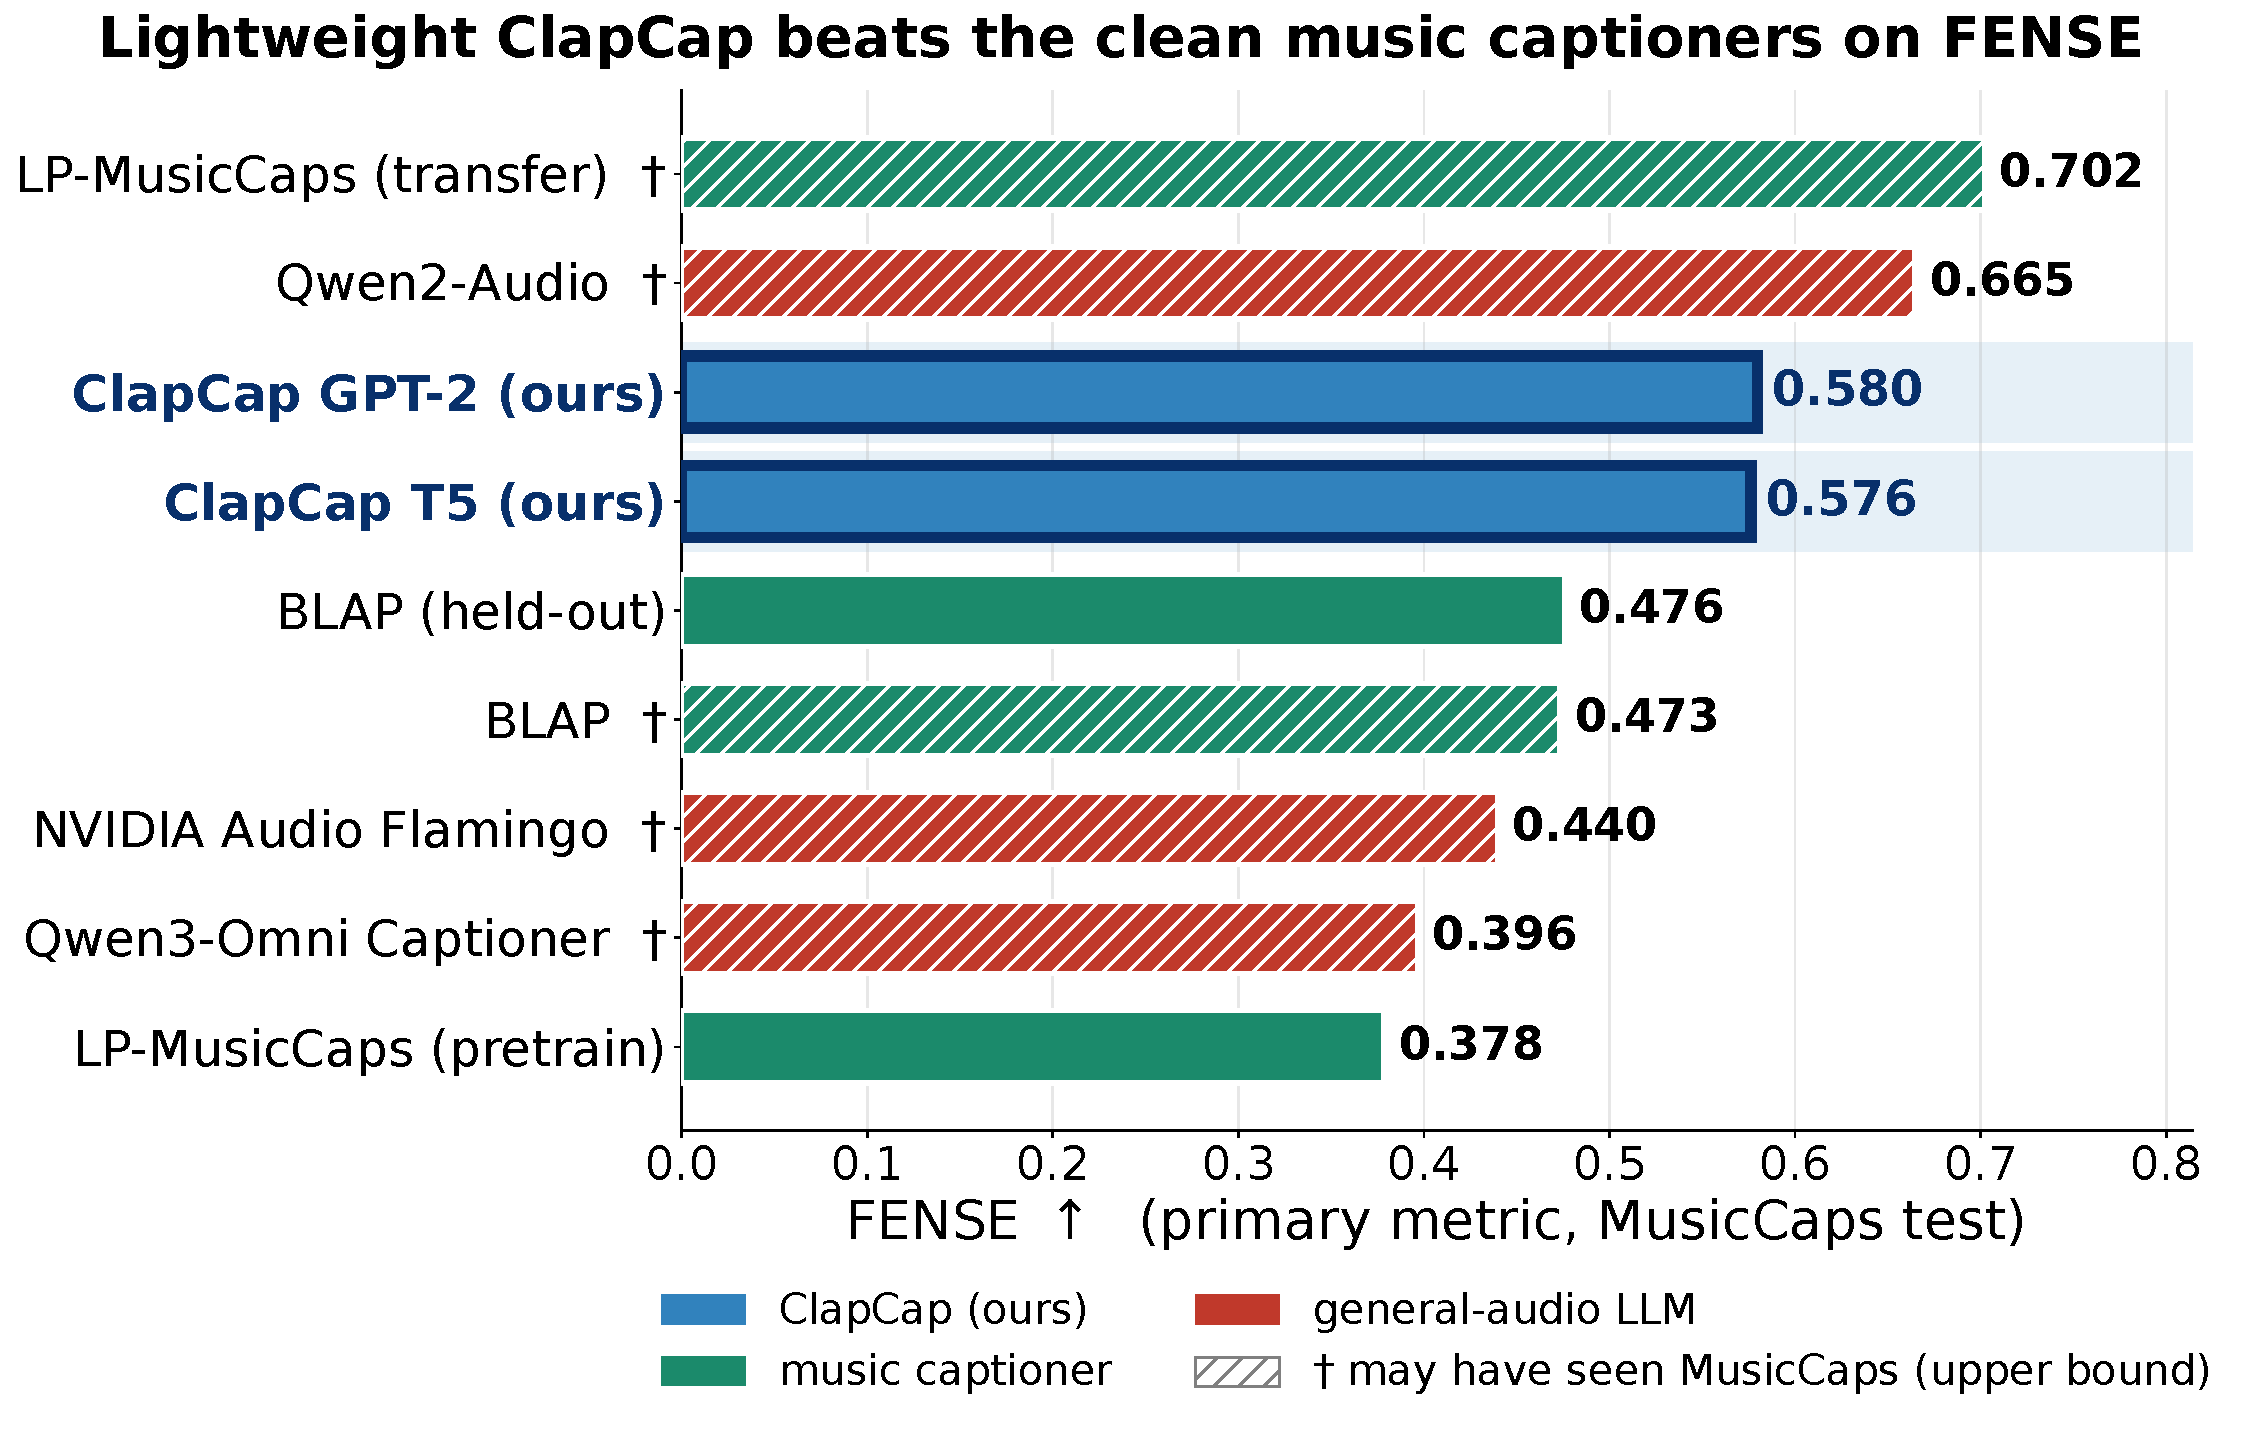
\includegraphics[width=\textwidth]{figures/fig_poster_fense.pdf}
\caption{Primary metric (\fense{}) on the shared MusicCaps test split: our lightweight pipeline
(GPT-2/T5, highlighted) against the zero-shot reference captioners. Hatched, daggered bars may
have seen MusicCaps in training (leakage upper bounds); for the two leaky music captioners the
clean held-out number is plotted instead. The pipeline's best decoding configuration is the
strongest leakage-free system.}
\label{fig:reference_fense}
\end{figure*}

\subsection{Human and LLM-judge evaluation}\label{sec:humaneval}

The automatic metrics rank GPT-2 and T5 as a statistical tie (Section~\ref{sec:baseline}). To
test whether that tie holds under human and model judgement, we ran a pairwise A-vs-B study.
Sixteen clip pairs (six GPT-2-best vs.\ the human MusicCaps reference, six GPT-2-best vs.\
T5-best, four reference-vs-mismatched-reference sanity checks) were each judged on two
questions: Q1 ``which caption is more accurate'' and Q2 ``which is less wrong'', with
A/B/tie/can't-tell responses. Pairwise comparison is used rather than absolute Likert scoring
because it gives more reliable inter-rater agreement on caption quality.

Ten lay listeners rated every pair; three were removed by a sanity check (agreement with the
obvious answer below $0.75$), leaving seven. The same pairs were scored by two language-model
panels under an identical rubric, both A/B orders averaged to cancel position bias, at
temperature zero with three repeats and logged model snapshots: an \emph{audio-grounded} panel
that hears the clip (Gemini~2.5~Pro, GPT-audio, Qwen3.5-Omni) and a larger
\emph{text-reference-only} panel that sees only the reference caption.

Lay raters are individually noisy but their \emph{consensus} tracks the audio-LLM panel.
Inter-human agreement is low (Fleiss $\kappa$ $0.131$ on Q1, $0.050$ on Q2), as expected for a
non-expert panel; the audio-LLM panel is more consistent ($0.392$/$0.486$). Crucially,
human-consensus versus audio-LLM-consensus agreement is substantial (Cohen $\kappa$ $0.643$ on
Q1, $0.696$ on Q2; raw agreement $80\%$/$86\%$). Win-rates point the same way in every pool
(Figure~\ref{fig:winrate}): the human reference beats GPT-2 ($69\%$ of human and $78\%$ of LLM
votes prefer the reference on Q1) and GPT-2 beats T5 ($72\%$ human / $71\%$ LLM). So the
pipeline does not beat the human reference, and the \fense{} tie between GPT-2 and T5 does
\emph{not} survive a preference test.

There is no human-versus-machine split in the per-judge agreement matrix: human consensus agrees
with the GPT-audio and Qwen judges (Cohen $\kappa$ up to $0.69$/$0.76$) more than the audio
judges agree among themselves, with Gemini~2.5~Pro the dissenting outlier. The dispersion is
\emph{within} the model panel, not between humans and models. The text-only panel is small (six
pairs, directional only) and one judge degenerates to always answering ``tie''; we report these
as limitations rather than findings.

\begin{figure*}[!t]\centering
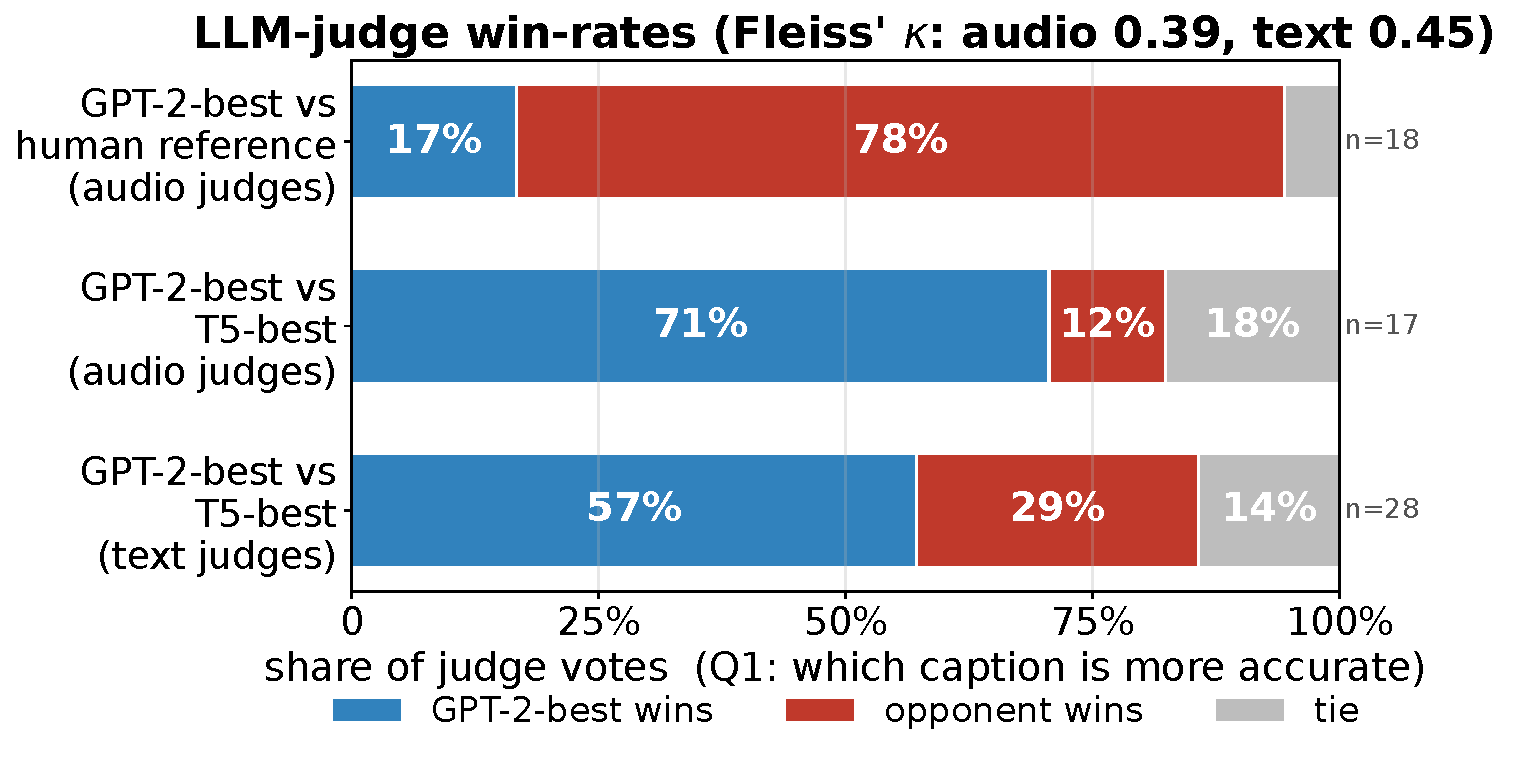
\includegraphics[width=\textwidth]{figures/fig_eval_winrate.pdf}
\caption{Pairwise A/B win-rates by rater pool. The reference-vs-GPT-2 block (the reference wins)
and the GPT-2-vs-T5 block (GPT-2 wins) point the same direction for the human, audio-LLM and
text-LLM pools. Bar counts $n$ are the decisive (non-tie) votes.}
\label{fig:winrate}
\end{figure*}

\section{Conclusion}\label{ch:conclusion}

We presented \sys{}, a controlled study of lightweight language models for \emph{music}
captioning via an audio adaptation of the ClipCap prefix recipe. Holding the frozen \clapenc{}
encoder, the projection, the data split and the evaluation fixed, a decoder-only and an
encoder--decoder LM are statistically indistinguishable at baseline once run-to-run variance is
measured; second-stage fine-tuning erases projection-level differences; and the largest decoding
lever improves the primary metric mostly by removing a fluency penalty rather than by improving
semantics. A reproducible vocalist bias turns out to be caption-prior amplification under
uncertain audio evidence. Swapping the general frontend for music-specialised encoders helps
only where the pretraining is pooled and joint audio--text. Against zero-shot reference
captioners on the same split, the pipeline at its best decoding setting is the strongest
leakage-free system, and a pairwise human and LLM-judge study corroborates the automatic
metrics while resolving the GPT-2/T5 tie in GPT-2's favour.

\textbf{Limitations.} The baseline encoder is trained on general audio, and whether a music
encoder helps more once the LM is also fine-tuned is left open. Several reference captioners may
have been trained on MusicCaps; we dagger them and report held-out scores where possible, but
their upper-bound numbers should not be read as clean. The human study uses ten lay listeners,
not music experts, with low individual agreement, so the agreement results are directional.
Scaling the LM is not free in this low-data regime ($\sim$4.5k clips): a billion-parameter
decoder fine-tuned end-to-end overfits within a single epoch --- the same overfitting
ClipCap~\cite{mokady2021clipcap} reports, amplified by scale. Finally, MusicCaps provides a
single reference per clip, which mechanically depresses n-gram metrics.

\textbf{Future work.} Extending the controlled comparison to billion-parameter decoders with a
gentler fine-tuning schedule; carrying the encoder ablation into Stage~2 and to a
LoRA-fine-tuned domain captioner; and audio-grounded metrics that score a caption against the
signal rather than a single text reference.

\begin{thebibliography}{99}

\bibitem{kim2019audiocaps}
C.~D. Kim, B.~Kim, H.~Lee, and G.~Kim,
``AudioCaps: Generating Captions for Audios in The Wild,'' in \emph{Proc. NAACL-HLT}, 2019.

\bibitem{drossos2020clotho}
K.~Drossos, S.~Lipping, and T.~Virtanen,
``Clotho: An Audio Captioning Dataset,'' in \emph{Proc. ICASSP}, 2020.

\bibitem{mokady2021clipcap}
R.~Mokady, A.~Hertz, and A.~H. Bermano,
``ClipCap: CLIP Prefix for Image Captioning,'' \emph{arXiv:2111.09734}, 2021.

\bibitem{wu2023clap}
Y.~Wu, K.~Chen, T.~Zhang, Y.~Hui, T.~Berg-Kirkpatrick, and S.~Dubnov,
``Large-Scale Contrastive Language-Audio Pretraining with Feature Fusion and
Keyword-to-Caption Augmentation,'' in \emph{Proc. ICASSP}, 2023.

\bibitem{deshmukh2023pengi}
S.~Deshmukh, B.~Elizalde, R.~Singh, and H.~Wang,
``Pengi: An Audio Language Model for Audio Tasks,'' in \emph{Proc. NeurIPS}, 2023.

\bibitem{agostinelli2023musiclm}
A.~Agostinelli, T.~I. Denk, Z.~Borsos, \emph{et al.},
``MusicLM: Generating Music From Text,'' \emph{arXiv:2301.11325}, 2023.

\bibitem{gemmeke2017audioset}
J.~F. Gemmeke, D.~P.~W. Ellis, D.~Freedman, A.~Jansen, W.~Lawrence, R.~C. Moore,
M.~Plakal, and M.~Ritter,
``Audio Set: An Ontology and Human-Labeled Dataset for Audio Events,'' in \emph{Proc. ICASSP},
2017.

\bibitem{doh2023lpmusiccaps}
S.~Doh, K.~Choi, J.~Lee, and J.~Nam,
``LP-MusicCaps: LLM-Based Pseudo Music Captioning,'' in \emph{Proc. ISMIR}, 2023.

\bibitem{lanzendorfer2025blap}
L.~A. Lanzendörfer, C.~Pinkl, N.~Perraudin, and R.~Wattenhofer,
``BLAP: Bootstrapping Language-Audio Pre-training for Music Captioning,'' in \emph{Proc. ICASSP},
2025.

\bibitem{chu2024qwen2audio}
Y.~Chu, J.~Xu, Q.~Yang, H.~Wei, X.~Wei, Z.~Guo, Y.~Leng, Y.~Lv, J.~He, J.~Lin, C.~Zhou, and
J.~Zhou,
``Qwen2-Audio Technical Report,'' \emph{arXiv:2407.10759}, 2024.

\bibitem{ghosh2026afnext}
S.~Ghosh, A.~Goel, K.~Jayakumar, L.~Koroshinadze, N.~Anand, \emph{et al.},
``Audio Flamingo Next: Next-Generation Open Audio-Language Models for Speech, Sound, and Music,''
\emph{arXiv:2604.10905}, 2026.

\bibitem{tang2024salmonn}
C.~Tang, W.~Yu, G.~Sun, \emph{et al.},
``SALMONN: Towards Generic Hearing Abilities for Large Language Models,'' in \emph{Proc. ICLR},
2024.

\bibitem{chen2022htsat}
K.~Chen, X.~Du, B.~Zhu, Z.~Ma, T.~Berg-Kirkpatrick, and S.~Dubnov,
``HTS-AT: A Hierarchical Token-Semantic Audio Transformer for Sound Classification and
Detection,'' in \emph{Proc. ICASSP}, 2022.

\bibitem{radford2019gpt2}
A.~Radford, J.~Wu, R.~Child, D.~Luan, D.~Amodei, and I.~Sutskever,
``Language Models are Unsupervised Multitask Learners,'' OpenAI, Tech. Rep., 2019.

\bibitem{raffel2020t5}
C.~Raffel, N.~Shazeer, A.~Roberts, \emph{et al.},
``Exploring the Limits of Transfer Learning with a Unified Text-to-Text Transformer,''
\emph{JMLR}, vol.~21, no.~140, 2020.

\bibitem{loshchilov2019adamw}
I.~Loshchilov and F.~Hutter,
``Decoupled Weight Decay Regularization,'' in \emph{Proc. ICLR}, 2019.

\bibitem{loshchilov2017sgdr}
I.~Loshchilov and F.~Hutter,
``SGDR: Stochastic Gradient Descent with Warm Restarts,'' in \emph{Proc. ICLR}, 2017.

\bibitem{akiba2019optuna}
T.~Akiba, S.~Sano, T.~Yanase, T.~Ohta, and M.~Koyama,
``Optuna: A Next-Generation Hyperparameter Optimization Framework,'' in \emph{Proc. ACM SIGKDD},
2019.

\bibitem{papineni2002bleu}
K.~Papineni, S.~Roukos, T.~Ward, and W.-J. Zhu,
``BLEU: a Method for Automatic Evaluation of Machine Translation,'' in \emph{Proc. ACL}, 2002.

\bibitem{banerjee2005meteor}
S.~Banerjee and A.~Lavie,
``METEOR: An Automatic Metric for MT Evaluation with Improved Correlation with Human
Judgments,'' in \emph{Proc. ACL Workshop on Intrinsic and Extrinsic Evaluation Measures for
Machine Translation and/or Summarization}, 2005.

\bibitem{lin2004rouge}
C.-Y. Lin,
``ROUGE: A Package for Automatic Evaluation of Summaries,'' in \emph{Text Summarization
Branches Out (ACL Workshop)}, 2004.

\bibitem{vedantam2015cider}
R.~Vedantam, C.~L. Zitnick, and D.~Parikh,
``CIDEr: Consensus-Based Image Description Evaluation,'' in \emph{Proc. CVPR}, 2015.

\bibitem{anderson2016spice}
P.~Anderson, B.~Fernando, M.~Johnson, and S.~Gould,
``SPICE: Semantic Propositional Image Caption Evaluation,'' in \emph{Proc. ECCV}, 2016.

\bibitem{liu2017spider}
S.~Liu, Z.~Zhu, N.~Ye, S.~Guadarrama, and K.~Murphy,
``Improved Image Captioning via Policy Gradient Optimization of SPIDEr,'' in \emph{Proc. ICCV},
2017.

\bibitem{zhou2022fense}
Z.~Zhou, Z.~Zhang, X.~Xu, \emph{et al.},
``Can Audio Captions Be Evaluated with Image Caption Metrics?,'' in \emph{Proc. ICASSP}, 2022.

\bibitem{reimers2019sbert}
N.~Reimers and I.~Gurevych,
``Sentence-BERT: Sentence Embeddings using Siamese BERT-Networks,'' in \emph{Proc.
EMNLP-IJCNLP}, 2019.

\bibitem{li2024mert}
Y.~Li, R.~Yuan, G.~Zhang, \emph{et al.},
``MERT: Acoustic Music Understanding Model with Large-Scale Self-Supervised Training,'' in
\emph{Proc. ICLR}, 2024.

\bibitem{won2024musicfm}
M.~Won, Y.-N. Hung, and D.~Le,
``A Foundation Model for Music Informatics,'' in \emph{Proc. ICASSP}, 2024.

\bibitem{zhu2025muq}
H.~Zhu, Y.~Zhou, H.~Chen, J.~Yu, Z.~Ma, R.~Gu, Y.~Luo, W.~Tan, and X.~Chen,
``MuQ: Self-Supervised Music Representation Learning with Mel Residual Vector Quantization,''
\emph{arXiv:2501.01108}, 2025.

\bibitem{xu2025qwen3omni}
J.~Xu, Z.~Guo, H.~Hu, Y.~Chu, X.~Wang, \emph{et al.},
``Qwen3-Omni Technical Report,'' \emph{arXiv:2509.17765}, 2025.

\end{thebibliography}

\end{document}
